\begin{frame}
    \frametitle{\problemtitle}
    \begin{itemize}
        \item<+-> \textbf{Problème:} Étant donné une distance $d$ et un angle $\alpha$ dans un triangle rectangle, trouver le double du deuxième côté adjacent.
        \begin{wrapfigure}{r}{5.5cm}
            \centering
            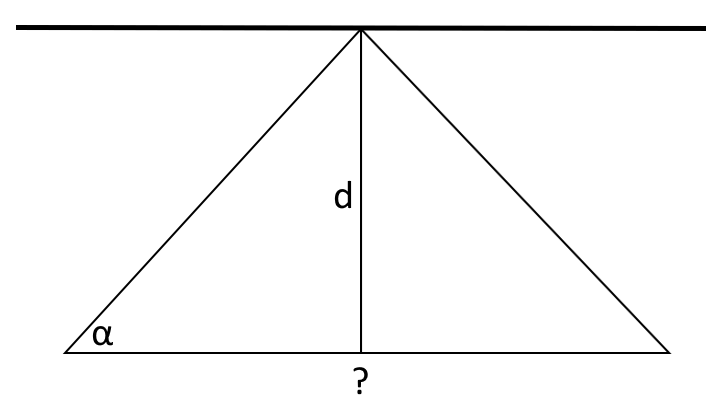
\includegraphics[width=5.5cm]{sol_mirror.jpg}
       \end{wrapfigure}
        \item<+-> Simple trigonométrie : $x=2d\cdot\tan(\mathsf{toDegree}(\alpha))$.
    \end{itemize}
    % \solvestats
\end{frame}
